\documentclass[tikz,border=10pt]{standalone}
\usepackage[T1]{fontenc}
\usepackage{lmodern}
\usetikzlibrary{positioning,arrows.meta,fit,backgrounds,shapes.geometric,calc}

\definecolor{coreindigo}{HTML}{3F51B5}
\definecolor{ifgreen}{HTML}{4CAF50}
\definecolor{adaptorange}{HTML}{FF9800}
\definecolor{syncpurple}{HTML}{9C27B0}
\definecolor{domteal}{HTML}{009688}
\definecolor{fsgray}{HTML}{757575}

\begin{document}
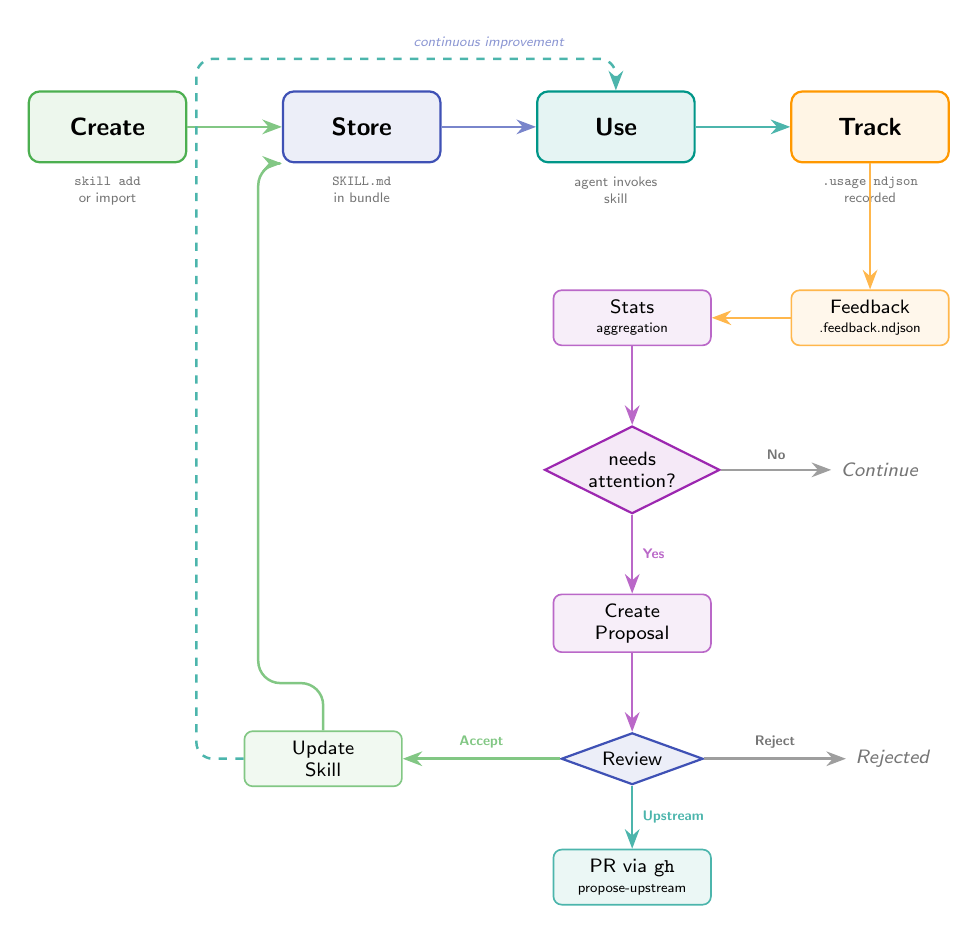
\begin{tikzpicture}[
    >=Stealth,
    every node/.style={font=\sffamily\small},
    phase/.style={
        draw=#1, fill=#1!10, rounded corners=4pt,
        minimum width=2cm, minimum height=0.9cm,
        line width=0.8pt, align=center, font=\sffamily\small\bfseries
    },
    detail/.style={
        font=\sffamily\tiny, text=fsgray, align=center
    },
    decision/.style={
        draw=#1, fill=#1!10, diamond, aspect=2,
        minimum width=1.8cm, inner sep=1pt,
        line width=0.8pt, font=\sffamily\scriptsize, align=center
    },
    action/.style={
        draw=#1!70, fill=#1!8, rounded corners=3pt,
        minimum width=2cm, minimum height=0.7cm,
        line width=0.6pt, font=\sffamily\scriptsize, align=center
    },
    arr/.style={->, thick, line width=0.9pt, color=#1!70},
    darr/.style={->, thick, line width=0.9pt, color=#1!70, dashed},
]

% === Main pipeline (top row) ===
\node[phase=ifgreen] (create) {Create};
\node[phase=coreindigo, right=1.2cm of create] (store) {Store};
\node[phase=domteal, right=1.2cm of store] (use) {Use};
\node[phase=adaptorange, right=1.2cm of use] (track) {Track};

% Detail labels
\node[detail, below=0.05cm of create.south] {\texttt{skill add}\\or import};
\node[detail, below=0.05cm of store.south] {\texttt{SKILL.md}\\in bundle};
\node[detail, below=0.05cm of use.south] {agent invokes\\skill};
\node[detail, below=0.05cm of track.south] {\texttt{.usage.ndjson}\\recorded};

% Main flow arrows
\draw[arr=ifgreen] (create) -- (store);
\draw[arr=coreindigo] (store) -- (use);
\draw[arr=domteal] (use) -- (track);

% === Feedback layer ===
\node[action=adaptorange, below=1.6cm of track] (feedback) {Feedback\\[-1pt]\tiny .feedback.ndjson};
\node[action=syncpurple, left=1cm of feedback] (stats) {Stats\\[-1pt]\tiny aggregation};

\draw[arr=adaptorange] (track.south) -- (feedback.north);
\draw[arr=adaptorange] (feedback) -- (stats);

% === Decision: needs attention? ===
\node[decision=syncpurple, below=1cm of stats] (attention) {needs\\attention?};
\draw[arr=syncpurple] (stats) -- (attention);

% No path: continue (exit)
\node[font=\sffamily\scriptsize\itshape, text=fsgray, right=1.4cm of attention] (cont) {Continue};
\draw[arr=fsgray] (attention.east) -- node[above, font=\sffamily\tiny\bfseries, text=fsgray] {No} (cont);

% Yes path: Proposal
\node[action=syncpurple, below=1cm of attention] (proposal) {Create\\Proposal};
\draw[arr=syncpurple] (attention.south) -- node[right, font=\sffamily\tiny\bfseries, text=syncpurple!70] {Yes} (proposal);

% Review decision
\node[decision=coreindigo, below=1cm of proposal] (review) {Review};
\draw[arr=syncpurple] (proposal) -- (review);

% Accept path
\node[action=ifgreen, left=2cm of review] (update) {Update\\Skill};
\draw[arr=ifgreen] (review.west) -- node[above, font=\sffamily\tiny\bfseries, text=ifgreen!70] {Accept} (update);

% Reject path
\node[font=\sffamily\scriptsize\itshape, text=fsgray, right=1.8cm of review] (reject) {Rejected};
\draw[arr=fsgray] (review.east) -- node[above, font=\sffamily\tiny\bfseries, text=fsgray] {Reject} (reject);

% Upstream path
\node[action=domteal, below=0.8cm of review] (upstream) {PR via \texttt{gh}\\[-1pt]\tiny propose-upstream};
\draw[arr=domteal] (review.south) -- node[right, font=\sffamily\tiny\bfseries, text=domteal!70] {Upstream} (upstream);

% === Continuous improvement loop ===
% Update -> back to Store
\draw[arr=ifgreen, rounded corners=8pt]
    (update.north) -- ++(0,0.6) -| ([xshift=-0.3cm]store.south west) -- (store.south west);

% Circular arrow from Use back (showing reuse)
\draw[darr=domteal, rounded corners=6pt]
    (update.west) -- ++(-0.6,0) |- ([yshift=0.4cm]use.north) -- (use.north);

% Loop annotation
\node[font=\sffamily\tiny\itshape, text=coreindigo!60,
    above=0.4cm of $(store.north)!0.5!(use.north)$] {continuous improvement};

\end{tikzpicture}
\end{document}
